\documentclass[addpoints]{exam}
  \makeatletter
  \expandafter\providecommand\expandafter*\csname ver@framed.sty\endcsname
  {2003/07/21 v0.8a Simulated by exam}
  \makeatother
\usepackage[top=1in, bottom=1in, left=1in, right=1in]{geometry}
\usepackage[utf8]{inputenc}
\usepackage[icelandic]{babel}
\usepackage[T1]{fontenc}
\usepackage[sc]{mathpazo}

\usepackage[parfill]{parskip}
\usepackage{booktabs,tabularx}
\usepackage{multirow}
\usepackage{multicol}
\usepackage{graphicx}
\usepackage{amsmath, amsfonts, amssymb, amsthm}
\usepackage{minted} %Minted and configuration
\usepackage{afterpage}
\usepackage{scrextend}

\usepackage[pdftex,bookmarks=true,colorlinks=true,pdfauthor={Eirikur Ernir Thorsteinsson},linkcolor=blue,urlcolor=blue]{hyperref}

\setcounter{secnumdepth}{-1} 
\hyphenpenalty=5000

\newcommand\blankpage{%
    \null
    \thispagestyle{empty}%
    \addtocounter{page}{-1}%
    \newpage}

\usemintedstyle{default}
\renewcommand{\theFancyVerbLine}{\sffamily \arabic{FancyVerbLine}}
\author{}
\date{}

\footer{}{}{}

\setcounter{secnumdepth}{-1} 

\qformat{\large \textbf Spurning \thequestion \phantom{M}(\totalpoints \phantom{l}stig) \hfill}
\renewcommand{\solutiontitle}{\noindent\textbf{Svar:}\par\noindent}
\renewcommand{\points}{stig}
\renewcommand{\questionshook}{\setlength{\itemsep}{0.5cm}}
\hqword{Spurning:}
\hpword{Stig í boði:}
\hsword{Stig:}
\htword{Samtals}

\title{TÖL105G Tölvunarfræði 1a - miðmisserispróf}
\author{}
\date{8. október 2016}

\pagestyle{headandfoot}
\firstpageheader{TÖL105G -\\ Tölvunarfræði 1a}{Miðmisserispróf}{8. október 2016}
\firstpagefooter{}{Bls. \thepage\ af \numpages}{}
\runningfooter{}{Bls. \thepage\ af \numpages}{}
\setlength{\columnsep}{0.5cm}

\printanswers
\begin{document}

% \thispagestyle{empty}
Fullt nafn: \vspace*{1mm} \hrule

\begin{center}
\begin{minipage}{.8\textwidth}
Á þessu prófi eru \numquestions\ spurningar sem samtals gefa 100 stig.
Ekki er dregið frá fyrir röng svör.
Skrifið svör í prófheftið.

Leyfileg hjálpargögn eru reiknivél og ein A4 blaðsíða af glósum.
\end{minipage}
\end{center}

\vspace{1cm}

\begin{questions}

\question Krossaspurningar. Merkið vandlega við réttan möguleika.

\begin{parts}
\part[5] Gefin er skipunin
\begin{minted}{matlab}
>> x = 0;
\end{minted}
í Matlab-skipanaglugganum. Af hvaða tagi verður breytan \texttt{x}?
\begin{checkboxes}
\choice \texttt{int32}
\choice \texttt{char}
\CorrectChoice \texttt{double}
\choice \texttt{logical}
\end{checkboxes}

\part[5]Hvert af eftirfarandi er \emph{löglegt} Matlab-breytuheiti?
\begin{checkboxes}
\choice \texttt{if}
\CorrectChoice \texttt{sum}
\choice \texttt{0}
\choice \texttt{númer}
\end{checkboxes}

\part[5] Gefnar eru skipanirnar
\begin{minted}{matlab}
>> v = [4 2 7 9 2];
>> v(v>5)
\end{minted}
í Matlab-skipanaglugganum. Hvert verður gildi breytunnar \texttt{ans} eftir að þær hafa verið keyrðar?
\begin{checkboxes}
\CorrectChoice \texttt{[7 9]}
\choice \texttt{[0 0 1 1 0]}
\choice \texttt{[3 4]}
\choice \texttt{[4 2 7 9 2]}
\end{checkboxes}

\part[5]Hvaða rökbreytu skilar yrðingin \texttt{1 > 3 > 2}?
\begin{checkboxes}
\choice \texttt{1}
\CorrectChoice \texttt{0}
\choice \texttt{[0 1]}
\choice Skilar engu, Matlab gefur villu.
\end{checkboxes}

\vspace*{1cm}
\gradetable[h][questions]
\newpage
% \vspace*{2cm}

\part[5] Hvað skrifar eftirfarandi kóðabútur út?
\begin{minted}{matlab}
a = true;
b = false;
if a == b || xor(a, b)
    a = b;
    b = a;
    if ~(a && b)
        a = ~b;
    end
end
disp([a b])
\end{minted}
\vspace{\baselineskip}
\begin{checkboxes}
\choice \texttt{0 0}
\CorrectChoice \texttt{1 0}
\choice \texttt{0 1}
\choice \texttt{1 1}
\end{checkboxes}

\part[5] Gefið er eftirfarandi fall:

\begin{minted}[frame=lines]{matlab}
function xplus(x)
x = x + 1;
end
\end{minted}

og eftirfarandi skipanir sem keyrðar eru í Matlab-skipanaglugganum:

\begin{minted}{matlab}
>> x = 1;
>> xplus(x)
\end{minted}

Hvert er gildi \texttt{x} í skipanaglugganum eftir að skipanirnar hafa verið keyrðar?

\begin{checkboxes}
\choice 0
\choice 2
\CorrectChoice 1
\choice \texttt{NaN}
\end{checkboxes}

\end{parts}

\newpage

\question Skrifið Matlab-skipanir (ein í hverjum lið) til að framkvæma eftirfarandi aðgerðir:
\begin{parts}
\part[3] Búið til $2 \times 4$ fylkið \texttt{m}, sem inniheldur jafndreifðar slembikommutölur á bilinu $]-3;3[$.
\vspace*{1.5cm}
\part[3] Búið til dálkvigurinn \texttt{v}, sem inniheldur lægstu tölu hverrar línu í \texttt{m}.
\vspace*{1.5cm}
\part[3] Búið til $2 \times 4$ rökfylkið \texttt{lm} sem inniheldur rökgildið ``satt'' þar sem tölugildi tilsvarandi staks í \texttt{m} er stærra en 2.
\vspace*{1.5cm}
\part[3] Breytið \texttt{m} í $4 \times 4$ fylki með því að skeyta afriti af fylkinu neðan á sjálft sig. (Þannig yrðu línur 1 og 3 alveg eins, sem og línur 2 og 4.)
\vspace*{1.5cm}
\part[3] Eyðið aftasta dálkinum úr \texttt{m}.
\vspace*{3cm}
\end{parts}

\begin{solution}

\begin{minted}{matlab}
>> m = rand(2,4)*(3-(-3))-3;
>> v = min(m')';
>> lm = abs(m) > 2;
>> m = [m ; m];
>> m(:,end) = [];
\end{minted}
\end{solution}

\question Í þessari spurningu skal notast við vigurkóðun.
\begin{parts}
\part[5] Gefinn er vigur \texttt{v} af heiltölum. Sýnið eina Matlab-skipun sem breytir \texttt{v} svo að hann innihaldi eingöngu tölur sem eru stærri en 10.
\vspace*{1.5cm}
\part[5] Gefinn er vigur \texttt{v} af jákvæðum heiltölum. Sýnið eina Matlab-skipun sem finnur stærstu tölu í \texttt{v} sem 3 gengur upp í (þ.e.a.s. stærstu tölu sem er margfeldi af 3).
\vspace*{1.5cm}
\end{parts}

\begin{solution}

\begin{minted}{matlab}
>> v = v(v > 10)
>> max(v(mod(v,3)==0))
\end{minted}

\end{solution}

\newpage
\question[5] Sýnið Matlab-skipanir sem teikna fallið $\sin(x^2)$ á bilinu $[0;10]$. Hafið ferilinn rauðan á litinn. Gagnapunktarnir skulu vera um það bil 1000 talsins. Myndin gæti þá litið svona út:
\begin{center}
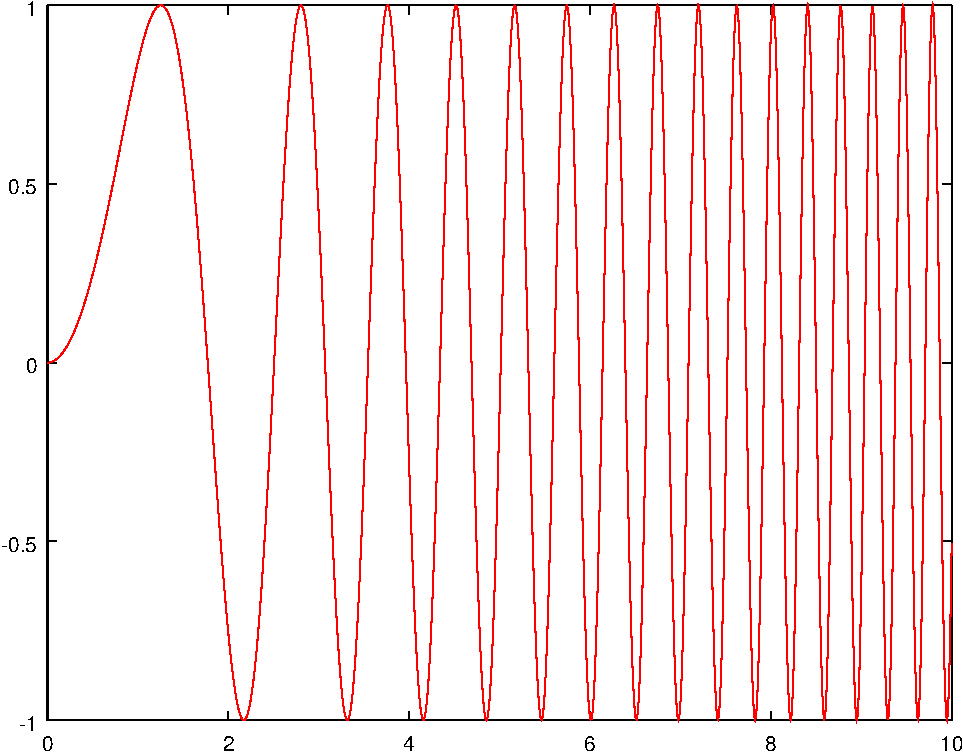
\includegraphics[width=0.75\textwidth]{Pics/sinx2}
\end{center}

\vspace{5cm}

\begin{solution}
 
\begin{minted}{matlab}
>> x = linspace(0,10,1000);
>> y = sin(x.^2);
>> plot(x, y, 'r')
\end{minted}

\end{solution}

\newpage
\question[10] Skrifið Matlab-skipanaskrána \texttt{spliffDonkGengja.m} sem skrifar út allar heiltölur frá 1 og upp í 100, með eftirfarandi undantekningum:

\begin{enumerate}
 \item Ef talan gengur upp í $2$ skal skrifa \texttt{Spliff} í stað tölunnar
 \item Ef talan gengur upp í $3$ skal skrifa \texttt{Donk} í stað tölunnar
 \item Ef talan gengur upp í bæði $2$ og $3$ skal skrifa \texttt{Gengja} í stað tölunnar
\end{enumerate}
Notið lykkju til að leysa þetta verkefni.

Dæmi um hluta af keyrslu forritsins:
\begin{minted}{matlab}
>> spliffDonkGengja
 1
Spliff
Donk
Spliff
 5
Gengja
 7
Spliff
Donk
Spliff
\end{minted}


\begin{solution}
\begin{minted}[frame=lines]{matlab}
n = 100;

for i = 1:n
  if mod(i,2) == 0 && mod(i,3) == 0
    disp('Gengja')
  elseif mod(i,2) == 0 
    disp('Spliff')
  elseif mod(i,3) == 0
    disp('Donk')
  else
    disp(i)  
  end
end
\end{minted}

\end{solution}

\newpage
\question[10]
Skrifið Matlab-skipanaskrá sem notar lykkju til að lesa inn tölur frá notanda. Forritið skal halda áfram að lesa inn tölur þar til summa allra talnanna sem lesnar hafa verið inn á þeim tímapunkti er orðin 100 eða hærri. Í hvert skipti sem lykkjan keyrist skal skrifa út hver núverandi summa er, með einum aukastaf. Þegar forritið lýkur keyrslu skal það skrifa út hver lokasumman varð, aftur með einum aukastaf.

Dæmi um mögulega keyrslu forritsins:

\begin{minted}{matlab}
Summa talnanna er 0.0
Vinsamlegast sláðu inn tölu: 25
Summa talnanna er 25.0
Vinsamlegast sláðu inn tölu: 25.22
Summa talnanna er 50.2
Vinsamlegast sláðu inn tölu: 50.78
Lokasumman varð 101.0
\end{minted}

\vspace*{6cm}

\begin{solution}

\begin{minted}{matlab}
total = 0;
while total <= 100
  fprintf('Summa talnanna er %.1f\n', total)
  total = total + input('Vinsamlegast sláðu inn tölu: ');
end
fprintf('Lokasumman varð %.1f\n', total)
\end{minted}
\end{solution}

\newpage
\question[10] Júlíus Sesar dulkóðaði skilaboð með því að hliðra hverjum staf um ákveðinn fjölda sæta í stafrófinu. 
Þannig hefði hann t.d. getað dulkóðað strenginn \texttt{JULIUS} með því að hliðra hverjum staf um þrjú sæti í (enska) stafrófinu og fengið út dulkóðunina \texttt{MXOLXV}.

Skrifið Matlab-fallið \texttt{encrypt} sem framkvæmir dulkóðun líka þeirri sem Sesar hefði getað framkvæmt hefði hann kunnað á Matlab. 

Fallið skal taka inn streng til dulkóðunar og jákvæða heiltölu $k$. Það skal skila streng sem hefur verið dulkóðaður með því að meðhöndla hvert tákn í inntaksstrengnum sem tölu, hækka töluna um $k$ og breyta tölunum aftur í tilsvarandi tákn.

Dæmi um mögulega keyrslu fallsins:
\begin{minted}{matlab}
>> encrypt('ENIGMA',1)
ans = FOJHNB
\end{minted}


\begin{solution}
 
\begin{minted}{matlab}
function c = encrypt(m, k)
c = char(m+k);
end
\end{minted}

\end{solution}

\newpage

\question[10] Skrifið Matlab-fall \texttt{isPartSorted} sem athugar hvort að vigur sé raðaður að hluta til. Fallið skal taka inn vigur $v$ og heiltölur $i$ og $j$, þar sem $1 \leq i \leq j \leq |v|$ (lengdin á $v$). 
Það skal skila tveimur breytum, annars vegar hlutvigrinum í $v$ sem byrjar í staki númer $i$ og endar í staki númer $j$ (að báðum stökum meðtöldum) og hins vegar rökbreytu sem er sönn ef hlutvigurinn er raðaður í stígandi röð, þ.e.a.s. hvert stak í hlutvigrinum er ekki stærra en þau stök sem á eftir koma, ef einhver eru.

Dæmi um mögulegar keyrslur fallsins þar sem inntaksbreyturnar eru taldar upp í röðinni $v$, $i$, $j$:

\begin{minted}{matlab}
>> [part, sorted] = isPartSorted([1, 2, 3, 4], 2, 3)
part =
   2   3
sorted =  1
>> [part, sorted] = isPartSorted([3, 4, 5, 1, 2], 2, 4)
part =
   4   5   1
sorted = 0
>> [part, sorted] = isPartSorted([3, 4, 2, 1], 3, 3)
part =  2
sorted =  1
\end{minted}

\begin{solution}
Einföld lausn:
\begin{minted}{matlab}
function [part, isSorted] = isPartSorted(v, i, j)
part = v(i:j);
isSorted = all(sort(part) == part);
end
\end{minted}
Hér er líka mjög eðlilegt að sjá lausnir sem nota lykkjur.
\end{solution}



% \question[10] Í hlutverkaleiknum Dungeons \& Dragons þarf oft að kasta fjölmörgum teningum til að ákvarða niðurstöður aðgerða.
% 
% Þegar persóna í leiknum heggur til annarrar þarf að kasta tuttugu hliða tening til að ákvarða hvort að höggið hitti. Ef niðurstaða tuttugu hliða teningsins er hærri en eða jöfn gefinni heiltölu $n$, þá hittir höggið.
% 
% Ef höggið hittir þarf að kasta upp á skaða, annars er skaðinn núll. Í þessu tilviki er skaðinn sú tala sem kemur upp á sex hliða teningi.
% 
% Skrifið Matlab-fallið \texttt{attack} sem notar slembitölur til að herma eftir einu höggi í Dungeons \& Dragons. Það skal taka inn eina jákvæða heiltölu $n$ sem táknar hversu há niðurstaða tuttugu hliða teningsins þarf að vera. Það skal skila tveimur breytum, annars vegar tölu sem táknar skaðann sem höggið gerir og hins vegar rökbreytu sem táknar hvort að höggið hitti yfir höfuð eða ekki.
% 
% Dæmi um mögulega keyrslu fallsins þar sem höggið hittir:
% \begin{minted}{matlab}
% >> n = 10; 
% >> [damage, hits] = attack(n)
% damage =  4
% hits =  1
% \end{minted}
% Dæmi um mögulega keyrslu fallsins þar sem höggið hittir ekki:
% \begin{minted}{matlab}
% >> [damage, hits] = attack(n)
% damage = 0
% hits = 0
% \end{minted}
% 
% \begin{solution}
%  
% \begin{minted}[frame=lines]{matlab}
% function [damage, hits] = attack(n)
% if randi([1 20]) < n
%   damage = 0;
% else
%   damage = randi([1 6]);
% end
% hits = damage > 0;
% end
% \end{minted}
% 
% \end{solution}


\end{questions}
\end{document}